\documentclass[crop,tikz]{standalone}
\usepackage{tikz}
\usetikzlibrary{shapes,arrows,positioning}
\begin{document}
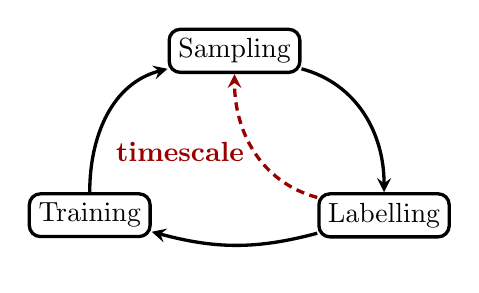
\begin{tikzpicture}[node distance=1.5cm and 0.2cm]
  \tikzstyle{proc} = [draw,rectangle,very thick,rounded corners]
  \tikzstyle{arrow} = [very thick,->,>=stealth]
  \tikzstyle{es} = [gray]
  \node (sampl) [proc] {Sampling};
  \node (train) [proc, below left =of sampl] {Training};
  \node (label) [proc, below right=of sampl] {Labelling};
  \draw [arrow] (label) to[out=195,in=-15]
  node[anchor=north](data){}
  (train);
  \draw [arrow] (train) to[out=90, in=195]
  node[sloped, anchor=south] (model) {}
  (sampl);
  \draw [arrow] (sampl) to[out=-15, in=90]
  node[sloped, anchor=south] (config) {}
  (label);
  \draw [arrow, red!60!black, densely dashed] (label) to[out=165,in=-90]
  node[midway,anchor=east, red!60!black] (time){\textbf{timescale}}
  (sampl);
\end{tikzpicture}
\end{document}
